
\section{2D/ 3D, DdQq models}

As was mentioned before, the velocities in the LGCA are discrete. The same idea applies to LBM, where the discretization of the velocities is similar and described with DdQq model. For example there are  such models as D2Q5, D2Q7, D2Q9, D2Q15, D3Q15, D3Q19 and D3Q27. D2Qq will be two-dimensional model, and D3Qq - three-dimensional.

D2Q9 is the model with 9 directions (one center for particles at rest, four directions along the axes and four diagonal directions, see left illustration in Fig. 3), D3Q27 model has 27 directions (one center, six directions along the axes, 12 combinations of two axes and 8 combinations of three axes, see right illustration in Fig. 3).

\begin{figure}[H]
  \centering
  \begin{subfigure}[h]{0.3\textwidth}
    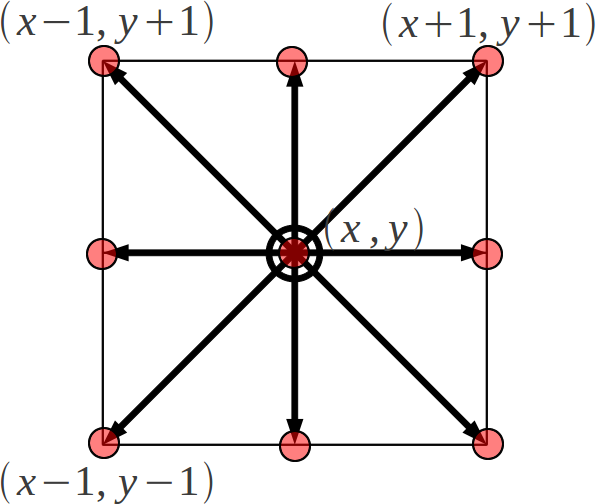
\includegraphics[width=\textwidth]{img/fig6-1.png}
  \end{subfigure}
  \begin{subfigure}[h]{0.3\textwidth}
    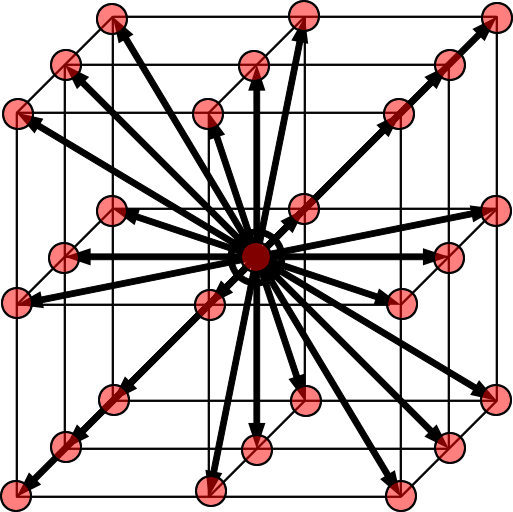
\includegraphics[width=\textwidth]{img/fig6-2.png}
  \end{subfigure}
  \caption{D2Q9 and D3Q27 velocity discretization models.}
\end{figure}

After discretizing the microscopic velocity space a system of N-1 equations is obtained. Such system is easier to solve than Navier-Stokes equations. N is the amount of probability densities (distribution functions). This system of equations is a hyperbolic. In figure 4 the streaming step on D2Q9 model, can be seen, which is described by the next functional:
\begin{equation}
f_i^{in}(\vec{r}+\vec{c}_{i}\Delta t, t+\Delta t) = f_i^{out}(\vec{r}, t)
\end{equation}

\begin{figure}[H]
  \centering
  \begin{subfigure}[h]{0.3\textwidth}
    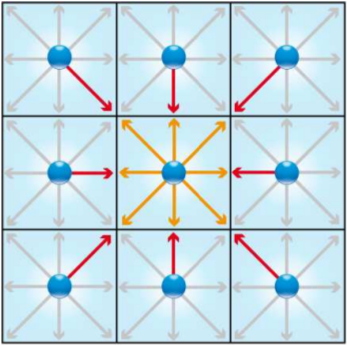
\includegraphics[width=\textwidth]{img/fig7-1.png}
  \end{subfigure}
  \begin{subfigure}[h]{0.3\textwidth}
    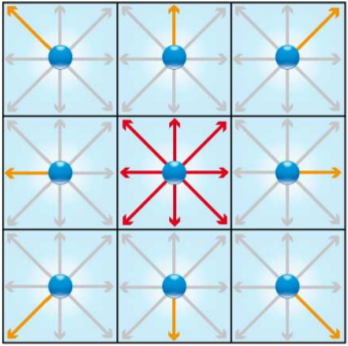
\includegraphics[width=\textwidth]{img/fig7-2.png}
  \end{subfigure}
  \caption{Streaming step [1].}
\end{figure}
